% Trotter layers by addition into a phase gradient
% REVTeX 4.2.  For submission to PRX Quantum use the class option prxquantum (REVTeX 4.2f or
% later); the prx option below gives the same layout on older installations.
\documentclass[aps,prx,twocolumn,superscriptaddress,nofootinbib,longbibliography]{revtex4-2}

\usepackage{amsmath,amssymb,amsthm}
\usepackage{graphicx}
\usepackage{braket}
\usepackage{booktabs}
\usepackage{xcolor}
\usepackage{tikz}
\usepackage[colorlinks=true,linkcolor=blue!50!black,citecolor=blue!50!black,urlcolor=blue!50!black]{hyperref}

\newtheorem{theorem}{Theorem}
\newtheorem{proposition}[theorem]{Proposition}
\newtheorem{lemma}[theorem]{Lemma}
\newtheorem{corollary}[theorem]{Corollary}
\theoremstyle{remark}
\newtheorem{remark}{Remark}

\newcommand{\AND}{\textup{\textsc{and}}}
\newcommand{\wt}{\operatorname{wt}}
\newcommand{\diam}[1]{\left\lVert #1\right\rVert_\diamond}
\newcommand{\Tc}{\mathcal{T}}

\begin{document}

\title{Trotter layers by addition into a phase gradient}

\author{Samuel J. Elman}
\affiliation{University of Technology Sydney, Sydney, Australia}

\date{\today}

\begin{abstract}
A Trotter step of a Hamiltonian with many distinct coefficients is a product of layers of
commuting Pauli rotations, and a fault-tolerant compilation synthesises each rotation on its
own. The best Clifford+T synthesis is a probabilistic mixture: about $0.53\log_2(1/\epsilon)$ T
gates for a channel within diamond error $\epsilon$, whatever the angle, and, as Bothe
\textit{et al.} have recently shown, far fewer when $\theta^2\lesssim\epsilon$. We ask whether a
catalytic phase-gradient register can do better. For one rotation it cannot: adding the angle
into a $b$-qubit gradient costs $b-2$ Toffoli gates, about $4\log_2(1/\epsilon)$ T gates. For a
layer it can. We write every angle of the layer in signed binary digits, reduce the digits
column by column with full adders, and add the one bit left in each column into the gradient
register once. A layer of $L$ rotations with $N$ signed digits then costs at most $4N+4(b-2)$ T
gates, plus one for each digit worth $\pi/4$, so a rotation by $\theta$ costs about
$\tfrac43\log_2(\theta/\Delta)$ T gates on a grid of spacing $\Delta$: the cost falls with the
angle across the whole range $\sqrt\epsilon\lesssim\theta\lesssim1$, where synthesis does not.
Rounding each angle at random between two grid points leaves only dephasing, so the grid can be
coarse, $\Delta\approx\sqrt{2\epsilon}$, and rounding onto a sparse pair of grid points costs
about $16\theta^2/\epsilon$ T gates in expectation when $\theta^2<\epsilon/2$. We prove the
counts and the errors and simulate every construction exactly, including the measurement-based
uncomputation. For Heisenberg chains of 64 spins in a random field, run to time 10 at total
errors of $10^{-3}$ and $10^{-1}$ with Trotter steps from $0.3$ to $10^{-6}$, the gradient
layers use $0.16$ to $0.88$ times the T gates of the angle-dependent synthesis of Bothe
\textit{et al.}, and never more; nearest rounding, which gives a unitary, uses $0.24$ to $0.51$
times the T gates of gridsynth. The price is ancillas: at most 589 for the randomised layers.
\end{abstract}

\maketitle

% ----------------------------------------------------------------------------------------------
\section{Introduction}

Product formulas are the simplest way to simulate a Hamiltonian
$H=\sum_j h_jP_j$, with $P_j$ Pauli strings, on a quantum
computer~\cite{Lloyd1996,Suzuki1991,Childs2021}. One step of length $\delta t$ is a product of
rotations $e^{-i\theta_jP_j}$ with $\theta_j=h_j\delta t$ (or a fixed fraction of it), arranged
in layers of commuting terms. In a fault-tolerant computation built from Clifford gates and T
gates the rotations are the expensive part, and the standard treatment synthesises each one to
its share of the error budget. Ross and Selinger's algorithm~\cite{RossSelinger2016} gives a
unitary with about $3\log_2(1/\epsilon)$ T gates. Kliuchnikov, Lauter, Minko, Paetznick and
Petit~\cite{Kliuchnikov2023} improved and combined the two ways of doing better, fallback
circuits with an ancilla and a measurement~\cite{Bocharov2015} and probabilistic mixtures of
approximations~\cite{Hastings2017,Campbell2017}: their mixed fallback protocol uses on average
$0.53\log_2(1/\epsilon)+4.86$ T gates for a channel within diamond error $\epsilon$, and their
mixed diagonal protocol, with no ancilla, $1.52\log_2(1/\epsilon)-0.01$. These counts do not
depend on the angle. That is odd for Trotter: as the step shrinks every angle shrinks with it,
and a rotation by $10^{-5}$ to precision $10^{-10}$ is charged the same as a rotation by one.

Bothe, S\"underhauf, Witham, Campbell and Blunt~\cite{Bothe2026} have recently removed this
oddity in part. In a mixture the cheap end can be the identity, so a small rotation is mostly
not applied at all, and when $\theta^2\lesssim\epsilon$ the expected cost falls to
$\tilde O(\theta^2/\epsilon)$; the T count of a Trotter circuit can then stay constant as the
step goes to zero. When $\theta^2\gg\epsilon$ their cost returns to that of
Ref.~\cite{Kliuchnikov2023}. Their cost formula, built on the protocols of
Ref.~\cite{Kliuchnikov2023}, is the comparison in this paper.

The question of this paper is whether a phase-gradient register helps. The register
$\ket{\Psi_b}=2^{-b/2}\sum_{y}e^{-2\pi iy/2^b}\ket{y}$ is an eigenstate of every addition
modulo $2^b$, so adding an integer $K$ into it applies the phase
$e^{2\pi iK/2^b}$ and leaves the register as it was~\cite{Kitaev2002,Gidney2018}. Additions
cost Toffoli gates, not rotations, and the register is prepared once for the whole
computation. Phase gradients are used this way for the quantum Fourier
transform~\cite{Nam2020}, for rotations by computed angles~\cite{Sanders2020}, and for
rotations by equal angles after Hamming-weight phasing~\cite{Gidney2018,Kivlichan2020}. For a
layer of rotations by distinct, fixed angles, the usual view is that each needs its own
controlled addition, about $b$ Toffoli gates, and so loses to synthesis.

Our answer has two halves.

\emph{For one rotation, no.} Adding $\theta$ into a $b$-qubit gradient costs $b-2-p_0$
Toffoli gates, $p_0$ the position of the lowest digit of the angle (Proposition~\ref{prop:one}),
about $4\log_2(1/\epsilon)$ T gates against gridsynth's $3.03\log_2(1/\epsilon)+5.4$, and, with
randomised rounding, about $2\log_2(1/\epsilon)$ against $0.53\log_2(1/\epsilon)+4.86$.

\emph{For a layer, yes.} The phase of a layer, $\sum_j\theta_jx_j$ on bits $x_j$, is a
weighted sum of bits, and once the angles are written in signed binary digits it is a sum of
columns of bits of equal weight. A column can be reduced with full adders, one Toffoli for every
bit removed, exactly as Hamming-weight phasing reduces one column of equal angles. After the
reduction one bit is left per column, and those bits are added into the gradient register once,
for $b-2$ Toffoli gates shared by the whole layer (Theorem~\ref{thm:layer}). A rotation then
costs about four T gates per signed digit of its angle. Its angle has about
$\tfrac13\log_2(\theta/\Delta)$ nonzero digits on a grid of spacing $\Delta$, so the cost falls
with the angle; and since rounding at random to the grid leaves only dephasing
(Lemma~\ref{lem:mix}), $\Delta$ can be as coarse as $\sqrt{2\epsilon}$. So the gradient's cost
falls with the angle over the whole range $\sqrt\epsilon\lesssim\theta\lesssim1$, the range in
which the cost of Ref.~\cite{Bothe2026} does not. For $\theta\lesssim\sqrt\epsilon$, rounding at
random onto a sparse pair of grid points gives the same $\theta^2/\epsilon$ scaling as
Ref.~\cite{Bothe2026} (Proposition~\ref{prop:tiny}). With batches sized by their digits rather
than by their rotations, the gradient stays the cheaper down to about $\sqrt\epsilon/10$; below
that, synthesis is, and both cost a few hundredths of a T gate per rotation.

Section~\ref{sec:setting} sets up the layer and the gradient. Section~\ref{sec:layer} gives the
circuit and its cost, Sec.~\ref{sec:rounding} the rounding and its error, and
Sec.~\ref{sec:numbers} the counts, against the angle-dependent formulas of
Ref.~\cite{Bothe2026} evaluated on the same angles, and against gridsynth, for single layers and
for Heisenberg chains run to a fixed time.
Section~\ref{sec:discussion} says what the comparison leaves out. The code, which compiles each
layer to Clifford gates, T gates and \AND{} gates and simulates it exactly, is
available~\cite{code}.

% ----------------------------------------------------------------------------------------------
\section{Setting}\label{sec:setting}

\paragraph*{A layer.}
A set of commuting Pauli strings can be mapped by a Clifford circuit to strings of $Z$s, and the
parity of a string of $Z$s can be computed into one qubit with CNOTs. So a layer is, up to
Clifford gates,
\begin{equation}\label{eq:layer}
  V(\boldsymbol\theta)=\prod_{j=1}^Le^{-i\theta_jZ_j}
  =e^{-i\sum_j\theta_j}\,\mathrm{diag}_x\,e^{2i\sum_j\theta_jx_j},
\end{equation}
with $Z_j$ acting on a bit $x_j$ (a qubit, or a computed parity) and
$Z_j=1-2x_j$. Several $Z_j$ may share a bit; nothing below needs them to be distinct. We drop
the global phase throughout. When the layer is controlled, as in phase estimation, the global
phase becomes a phase on the control and costs one more addition.

\paragraph*{The gradient.}
For $b\ge4$ let $\ket{\Psi_b}=2^{-b/2}\sum_{y=0}^{2^b-1}e^{-2\pi iy/2^b}\ket{y}$. If a circuit
$A$ maps $\ket{x}\ket{y}$ to $\ket{x}\ket{y+f(x)\bmod2^b}$, then
\begin{equation}\label{eq:kickback}
  A\ket{x}\ket{\Psi_b}=e^{2\pi if(x)/2^b}\ket{x}\ket{\Psi_b}.
\end{equation}
The register is a product state: qubit $k$ is $(\ket0+e^{-2\pi i2^k/2^b}\ket1)/\sqrt2$, so the top
qubit is $\ket-$, the next $S^\dagger\ket+$, the next $T^\dagger\ket+$. It is prepared once, with
$b-3$ synthesised rotations, and returned unchanged by every addition. Its preparation error
enters once, not once per use, because the whole computation is a fixed channel applied to the
input and the register. On the gradient, the rotation $e^{-i\theta Z}$ on a bit $x$ is the
addition of $Kx$ with
\begin{equation}\label{eq:grid}
  \theta=K\Delta,\qquad \Delta=\pi/2^b,
\end{equation}
so the $Z$ angles live on a grid of spacing $\Delta$.

\paragraph*{Gates and costs.}
We count T gates. The circuits use Clifford gates, T gates, and the logical \AND{} of
Jones~\cite{Jones2013} and Gidney~\cite{Gidney2018}: a Toffoli onto a fresh qubit, four T
gates, uncomputed by an $X$-basis measurement and a CZ conditioned on the outcome, with no T
gate. Every \AND{} below is uncomputed this way, so a Toffoli costs four T gates once. In a
surface-code factory a Toffoli is cheaper than four T gates~\cite{Gidney2019}; counting
four is the conservative choice for the gradient.

\paragraph*{Errors.}
Errors are diamond distances~\cite{Aharonov1998}, per rotation, as in the synthesis
literature. For two unitaries that differ by $e^{-i\delta Z}$ the distance is $2|\sin\delta|$.
Unitary errors add along a circuit, and so do channel errors in the diamond norm.

\paragraph*{Signed digits.}
Every integer has a unique non-adjacent form (NAF) $K=\sum_pd_p2^p$ with $d_p\in\{-1,0,1\}$
and no two adjacent digits nonzero~\cite{Reitwiesner1960}. It has the fewest nonzero digits of
any signed-digit expansion of $K$~\cite{Reitwiesner1960,Arno1993}; we write $\wt(K)$ for their
number. An integer below $2^\ell$ in magnitude has $\wt(K)\le\lceil(\ell+1)/2\rceil$, and a
random one about $\ell/3$~\cite{Arno1993}. Modulo $2^b$ we expand the representative of $K$ in
$(-2^{b-1},2^{b-1}]$; a digit at position $b$ would be worth a whole turn and is dropped.

% ----------------------------------------------------------------------------------------------
\section{One addition per layer}\label{sec:layer}

\begin{figure}[t]
\centering
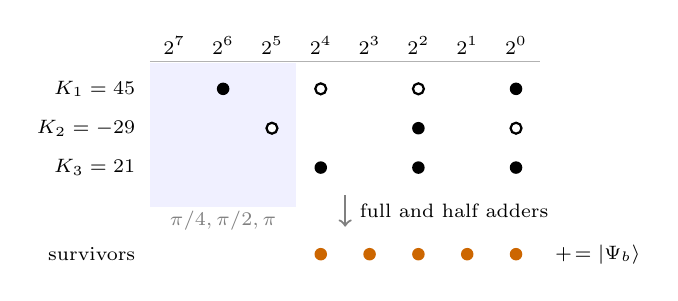
\begin{tikzpicture}[x=0.62cm,y=0.5cm,
  pdot/.style={circle,fill=black,inner sep=1.6pt},
  neg/.style={circle,draw=black,fill=white,inner sep=1.4pt,thick},
  sur/.style={circle,fill=orange!80!black,inner sep=1.6pt}]
  \foreach \p/\lab in {0/0,1/1,2/2,3/3,4/4,5/5,6/6,7/7}{
    \node[font=\scriptsize] at (7-\p,4.7) {$2^{\lab}$};}
  \draw[gray!60] (-0.5,4.3) -- (7.5,4.3);
  \fill[blue!6] (-0.5,4.25) rectangle (2.5,0.6);
  \node[font=\scriptsize,gray] at (1,0.25) {$\pi/4,\pi/2,\pi$};
  \node[font=\scriptsize,anchor=east] at (-0.6,3.6) {$K_1=45$};
  \node[font=\scriptsize,anchor=east] at (-0.6,2.6) {$K_2=-29$};
  \node[font=\scriptsize,anchor=east] at (-0.6,1.6) {$K_3=21$};
  % K1 = 45 = 64 - 16 - 4 + 1 : NAF digits 6:+,4:-,2:-,0:+
  \node[pdot] at (7-0,3.6) {}; \node[neg] at (7-2,3.6) {}; \node[neg] at (7-4,3.6) {};
  \node[pdot] at (7-6,3.6) {};
  % K2 = -29 = -32 + 4 - 1 : digits 5:-, 2:+, 0:-
  \node[neg] at (7-0,2.6) {}; \node[pdot] at (7-2,2.6) {}; \node[neg] at (7-5,2.6) {};
  % K3 = 21 = 16 + 4 + 1
  \node[pdot] at (7-0,1.6) {}; \node[pdot] at (7-2,1.6) {}; \node[pdot] at (7-4,1.6) {};
  \draw[->,thick,gray] (3.5,0.9) -- (3.5,0.1);
  \node[font=\scriptsize,anchor=west] at (3.6,0.5) {full and half adders};
  \foreach \p in {0,1,2,3,4}{\node[sur] at (7-\p,-0.6) {};}
  \node[font=\scriptsize,anchor=west] at (7.6,-0.6) {$+\!=\ket{\Psi_b}$};
  \node[font=\scriptsize,anchor=east] at (-0.6,-0.6) {survivors};
\end{tikzpicture}
\caption{The phase of a layer as columns of bits ($b=8$). Each rotation contributes one bit per
nonzero signed digit of its angle: a filled dot is $x_j$, an open dot is $\bar x_j$ (a digit
$-1$, $-x=\bar x-1$). Columns $b-3$, $b-2$, $b-1$ (shaded) are worth $\pi/4$, $\pi/2$ and
$\pi$ per bit and get T, S and Z gates directly. The other columns are reduced from the right
to one bit each, carries moving left, with one \AND{} per full or half adder, and the
survivors are added into the gradient register as one integer.}
\label{fig:columns}
\end{figure}

Write each $K_j$ in signed digits and each digit $d_{jp}=-1$ on a bit $x$ as the bit $\bar x$
with the constant $-1$. Then
\begin{equation}\label{eq:columns}
  \sum_jK_jx_j+C\equiv\sum_{p=0}^{b-1}2^p\,\bigl|\{\text{ones in column }p\}\bigr|
  \pmod{2^b},
\end{equation}
where column $p$ holds one bit, $x_j$ or $\bar x_j$, for each nonzero digit $d_{jp}$, and $C$ is
the sum of $2^p$ over the digits $-1$ (Fig.~\ref{fig:columns}). The constant only changes the
global phase. The circuit has three parts.

\emph{Compute.} Copy the bit of each digit at a position $p\le b-4$ into a fresh qubit in
column $p$ (a CNOT, and an X for a digit $-1$). Then, for $p=0,1,\dots,b-4$ in turn, reduce
column $p$ to at most one bit. While it holds three or more bits, replace three of them, $a$,
$a'$ and $c$, by their sum $a\oplus a'\oplus c$ in column $p$ and their majority in column
$p+1$:
\begin{equation}
  a+a'+c=(a\oplus a'\oplus c)+2\,\mathrm{maj}(a,a',c),
\end{equation}
computed in place with CNOTs and one \AND{}, since
$\mathrm{maj}(a,a',c)=a\oplus(a\oplus a')(a\oplus c)$. When two bits are left, replace them by
$a\oplus a'$ in column $p$ and $aa'$ in column $p+1$, again one \AND{}.

\emph{Phase.} Apply T, S and Z to every bit in columns $b-3$, $b-2$ and $b-1$: the bits of the
digits there, and the carries out of column $b-4$. Add the survivors, one bit in each column
$p\le b-4$, as an integer $S<2^{b-3}$ into the gradient register, with Gidney's
adder~\cite{Gidney2018}. Because the top qubit of the register is $\ket-$, the carry into it is
applied as a phase and never computed.

\emph{Uncompute.} Run the compute part backwards, each \AND{} undone by measurement.

\begin{theorem}[a layer]\label{thm:layer}
Let $b\ge4$ and let $K_1,\dots,K_L$ be integers whose signed-digit expansions modulo $2^b$ have
$N$ nonzero digits at positions $p\le b-4$ and $N_3$ at position $b-3$. The circuit above,
with one copy of $\ket{\Psi_b}$, implements
$\ket{x}\mapsto e^{2\pi i(\sum_jK_jx_j+C)/2^b}\ket{x}$ exactly, returns the register and every
ancilla unchanged, and uses at most $N+b-2$ \AND{} gates and $N_3+c$ further T gates, where
$c\le N/2$ is the number of carries out of column $b-4$. Its T count is at most
\begin{equation}\label{eq:tcount}
  \Tc\le4N+N_3+4(b-2).
\end{equation}
It uses at most $2N+b-2$ ancillas besides the register, plus one for each digit $-1$ in the top
three columns.
\end{theorem}

\begin{proof}
\emph{Correctness.} Each full or half adder keeps the right-hand side of
Eq.~\eqref{eq:columns} fixed, since it replaces bits of total value $a+a'+c$ (or $a+a'$) in
column $p$ by bits of the same value in columns $p$ and $p+1$. The T, S and Z gates on columns
$b-3$, $b-2$ and $b-1$ apply $e^{2\pi i2^p/2^b}$ for each bit set there, and the addition
applies $e^{2\pi iS/2^b}$ by Eq.~\eqref{eq:kickback}. Together they apply
$e^{2\pi i(\sum_jK_jx_j+C)/2^b}$. The compute part is a reversible classical map with all
inputs kept (each \AND{} target and each copy is fresh), so running it backwards restores every
ancilla to $\ket0$; the measured uncompute of an \AND{} is exact~\cite{Gidney2018}.

\emph{Counts.} Let column $p$ receive $n_p$ digit bits and $c_p$ carries, $c_0=0$, and
$m_p=n_p+c_p$. A full adder removes two bits from the column and a half adder one, and each
sends one carry on, so reducing $m_p$ bits to one takes $\lfloor m_p/2\rfloor$ adders and
$c_{p+1}=\lfloor m_p/2\rfloor$. The \AND{}s of the compute part number
$A=\sum_{p=0}^{b-4}c_{p+1}$, and
\begin{equation}
  A\le\sum_{p=0}^{b-4}\frac{n_p+c_p}{2}=\frac{N+A-c_{b-3}}{2},
\end{equation}
so $A\le N-c_{b-3}$. The adder for $S$ has one \AND{} per carry position from the lowest
survivor $p_0$ to $b-3$, that is $b-2-p_0\le b-2$, and its top carry is a phase. The direct
gates add $N_3+c_{b-3}$ T gates (S and Z are Clifford). So
$\Tc\le4(N-c_{b-3})+4(b-2)+N_3+c_{b-3}\le4N+N_3+4(b-2)$.
\emph{Ancillas:} $N$ copies, $A\le N$ carries, at most $b-2$ in the adder, and a copy for each
negated top digit.
\end{proof}

Hamming-weight phasing~\cite{Gidney2018,Kivlichan2020} is the case of one column: $L$ bits
that share an angle are added into a $\lfloor\log_2L\rfloor+1$-bit count with about $L$
\AND{}s, and the count is rotated. The construction above is the same reduction applied to
every column of the angles' digits at once, the reduction of a multiplier's partial
products~\cite{Wallace1964}, with the gradient register as the final adder. Equal angles can be
combined with it: our code first sums a class of bits that share an angle into its Hamming
weight $W=\sum_kw_k2^k$, and then treats each bit $w_k$ as one rotation, by $2^k\theta$ or by
its own rounding of it.

\begin{proposition}[one rotation]\label{prop:one}
For $L=1$ and $K$ with lowest nonzero digit at position $p_0\le b-4$, the circuit has no adders
in the compute part and $b-2-p_0$ \AND{}s in the addition, so $\Tc=4(b-2-p_0)+N_3$.
\end{proposition}

\begin{proof}
Each column holds at most one bit, so the compute part only copies. The rest is the count of
the adder in the proof of Theorem~\ref{thm:layer}.
\end{proof}

The proposition is also the cost of the controlled constant addition that rotates one qubit:
fanning the bit out to the positions of the digits of $K$ with CNOTs makes it an ordinary
addition, so the control costs nothing extra. For a generic angle $p_0$ is small, and at the
error $\epsilon$ of a unitary rounding (Sec.~\ref{sec:rounding}), $b=\lceil\log_2(\pi/\epsilon)
\rceil$ and $\Tc\approx4\log_2(1/\epsilon)$, against $3.03\log_2(1/\epsilon)+5.4$ for gridsynth.
For channels the comparison is worse: $\Tc\approx2\log_2(1/\epsilon)$ against
$0.53\log_2(1/\epsilon)+4.86$. A phase gradient on its own does not make an isolated rotation
cheaper. What it does is make the $b-2$ Toffoli gates of the carry chain a cost per layer
rather than per rotation.

\begin{corollary}[cost per rotation]\label{cor:per}
Split a layer into batches of $B$ rotations, each with its own compute part and addition. A
rotation costs at most $4\wt(K)+4(b-2)/B+[\text{digit at }b-3]$ T gates, its share of the
addition included. If $|\theta|\le2^\ell\Delta$, then $\wt(K)\le\lceil(\ell+2)/2\rceil$.
\end{corollary}

So the cost per rotation is set by the number of nonzero digits of its angle, which grows as
$\log_2(\theta/\Delta)$ and not as $\log_2(1/\Delta)$: the digits below position $\log_2\Delta$
are not there, and those above $\log_2\theta$ are zero.

% ----------------------------------------------------------------------------------------------
\section{Rounding}\label{sec:rounding}

The integers $K_j$ approximate $\theta_j/\Delta$. There are two ways to choose them.

\paragraph*{Nearest.} $K=\mathrm{round}(\theta/\Delta)$ leaves a rotation error $|\delta|\le
\Delta/2$, a diamond error $2\sin(\Delta/2)\le\Delta$. A per-rotation error $\epsilon$ needs
the least $b$ with $2\sin(\pi/2^{b+1})\le\epsilon$, $b\approx\log_2(\pi/\epsilon)$.

\paragraph*{Randomised.} Choose between the two neighbours at random, with the probability that
cancels the coherent part of the error.

\begin{lemma}[randomised rounding]\label{lem:mix}
Let $u,v\ge0$, $0<u+v\le\pi/2$, and let $q=\sin2u/(\sin2u+\sin2v)$. The channel that applies
$e^{-i(\theta+v)Z}$ with probability $q$ and $e^{-i(\theta-u)Z}$ with probability $1-q$ is
$\mathcal U_\theta\circ\mathcal D_p$, where $\mathcal U_\theta$ is the rotation by $\theta$,
$\mathcal D_p(\rho)=(1-p)\rho+pZ\rho Z$, and
\begin{equation}
  p=\frac{\sin u\sin v}{\cos(u-v)}=\frac12\Bigl(1-\frac{\cos(u+v)}{\cos(u-v)}\Bigr)
  \le\sin^2\frac{u+v}{2}.
\end{equation}
Its diamond distance from $\mathcal U_\theta$ is $2p$.
\end{lemma}

\begin{proof}
For a rotation by $\delta$ after $\mathcal U_\theta$,
$e^{-i\delta Z}\rho e^{i\delta Z}=\cos^2\!\delta\,\rho+\sin^2\!\delta\,Z\rho Z
-\tfrac i2\sin2\delta\,[Z,\rho]$. Averaged over $\delta=v$ with probability $q$ and
$\delta=-u$ with probability $1-q$, the commutator term has weight
$q\sin2v-(1-q)\sin2u=0$, and the rest is $\mathcal D_p$ with
$p=(1-q)\sin^2u+q\sin^2v$. Substituting $q$ and using $\sin2x=2\sin x\cos x$ gives
$p=\sin u\sin v\,\sin(u+v)/[\sin(u+v)\cos(u-v)]$, and $2\sin u\sin v=\cos(u-v)-\cos(u+v)$
gives the second form; it is largest at $u=v$. Finally
$\diam{\mathcal D_p-\mathrm{id}}=2p\,\diam{\tfrac12(Z\cdot Z-\mathrm{id})}=2p$, the norm
attained on a maximally entangled input.
\end{proof}

With $u+v=\Delta$ the dephasing is at most $\sin^2(\Delta/2)$ and the error at most
$2\sin^2(\Delta/2)\approx\Delta^2/2$: the grid can be coarser, $b\approx\tfrac12\log_2(\pi^2/
2\epsilon)$, half the bits of nearest rounding. This is the mixing of
Hastings~\cite{Hastings2017} and Campbell~\cite{Campbell2017} applied to the grid, where it is
exact: the two neighbours differ only in their $Z$ angle, so no off-axis error survives the
average. In a layer the roundings are drawn independently, the circuit compiled for each draw
implements its rotations exactly (Theorem~\ref{thm:layer}), and the averaged channel is
$V(\boldsymbol\theta)$ followed by independent dephasings by the operators $Z_j$. These commute,
so the layer's error is at most $\sum_j2p_j$. The same holds for a rotation of a computed bit,
such as a bit $w_k$ of a Hamming weight: $(-1)^{w_k(x)}$ is a diagonal involution and the
proof is unchanged. The draws are classical and made at compile time; each Trotter step draws
afresh.

\paragraph*{Sparse pairs.}
Nothing in Lemma~\ref{lem:mix} needs $u$ and $v$ to be one grid step. Rounding onto a farther
pair $K_-<\theta/\Delta<K_+$ costs more dephasing and may cost fewer digits. Our code searches,
for each weight $w$, the nearest grid points of weight at most $w$ on either side and the
farthest partner each can have within the dephasing budget, and takes the pair with the least
expected weight $(1-q)\wt(K_-)+q\wt(K_+)$; the adjacent pair is among the candidates. For
moderate angles this saves little (Sec.~\ref{sec:numbers}). For small angles it is what matters.

\begin{proposition}[small angles]\label{prop:tiny}
Let $\theta>0$, $\theta^2\le\epsilon/2$ and $\sin^2(\Delta/2)\le\epsilon/2$. Let $D=2^k\Delta$
with $k$ the largest integer for which $D\ge\theta$ and the pair $\{0,D\}$ has dephasing at most
$\epsilon/2$, and suppose $2D\le\pi/4$. Randomised rounding onto $\{0,D\}$ has error at most
$\epsilon$, and uses one digit with probability
\begin{equation}
  q\le\frac{4\theta^2}{\epsilon}\cdot\frac{1}{\cos2D\,(1-2D^2/3)}
\end{equation}
and none otherwise. Its expected T count is at most $4q$, that is $16\theta^2/\epsilon$ to
leading order, plus its share of an addition that is needed only if some digit of the batch is
drawn.
\end{proposition}

\begin{proof}
Such a $k$ exists: let $D_0$ be the least $2^j\Delta\ge\theta$. If $D_0=\Delta$ the dephasing of
$\{0,D_0\}$ is at most $\sin^2(\Delta/2)\le\epsilon/2$ by Lemma~\ref{lem:mix}; otherwise
$D_0<2\theta$ and it is at most $\sin^2(D_0/2)<\theta^2\le\epsilon/2$. By maximality the pair
$\{0,2D\}$ has dephasing above $\epsilon/2$:
$\sin\theta\sin(2D-\theta)>\tfrac\epsilon2\cos(2D-2\theta)\ge\tfrac\epsilon2\cos2D$, and with
$\sin x\le x$, $D>\epsilon\cos2D/(4\theta)$. Next, $q=\sin2\theta/(\sin2\theta+\sin2(D-\theta))$,
and since $\sin a+\sin b\ge\sin(a+b)$ for $a,b\ge0$, $a+b\le\pi$,
$\sin2\theta+\sin2(D-\theta)\ge\sin2D\ge2D(1-2D^2/3)$. So $q\le\theta/[D(1-2D^2/3)]$, and the
bound on $D$ gives the result. The error is $2p\le\epsilon$ by Lemma~\ref{lem:mix}. A drawn digit
costs at most four T gates: by the proof of Theorem~\ref{thm:layer} it adds at most one \AND{}
to the compute part, or one T gate if it lands in column $b-3$.
\end{proof}

When $\theta<\epsilon/2$ the rotation can be dropped altogether, at error $2\sin\theta<
\epsilon$. Proposition~\ref{prop:tiny} is the gradient's version of the small-angle regime of
Ref.~\cite{Bothe2026}: in both, the cost of a rotation with $\theta^2\ll\epsilon$ is of order
$\theta^2/\epsilon$, because a rotation that small is mostly not applied. The gradient's
expected digit cost, $16\theta^2/\epsilon$, is below theirs, which at $\theta=\sqrt\epsilon/10$
is between $30$ and $50$ times $\theta^2/\epsilon$; what decides the comparison there is the
share of the addition, paid by a batch only if it draws a digit (Sec.~\ref{sec:numbers}). Between the two regimes, for $\epsilon\ll\theta^2$, the
gradient's cost is about $\tfrac43\log_2(\theta/\Delta)\approx\tfrac23\log_2(\theta^2/2\epsilon)$
T gates with randomised rounding, and still falls with the angle; theirs is
$\min\{0.53\log_2(1/\epsilon)+4.86,\ \dots\}$ and in this regime equal to the first term.

\paragraph*{Sparse nearest rounding.}
The same search for nearest rounding (the lightest grid point within the error, on a grid finer
than needed) changes the mean weight by less than one per cent for every angle scale we tried,
and we do not use it.

% ----------------------------------------------------------------------------------------------
\section{Counts}\label{sec:numbers}

\paragraph*{The gradient.}
The gradient layers are compiled by our code to Clifford gates, T gates and \AND{}s, and every
compiled circuit is checked by exact simulation: with the system in each basis state and the
gradient register in $\ket{\Psi_b}$, the circuit maps basis states to phases times basis states,
so all $2^b$ branches of the register can be followed at once and the output compared with
$e^{2\pi i(f(x)+C)/2^b}\ket{x}\ket{\Psi_b}$, ancillas returned to $\ket0$. The tests do this
for 100 random layers with up to eight bits and $b\le10$, including equal-angle classes and
per-bit roundings, and a full state-vector simulation with the \AND{}s uncomputed by actual $X$
measurements with random outcomes agrees to $10^{-16}$. The bound~\eqref{eq:tcount} is checked
on every layer counted below.

The layers are split into batches of at most $D=256$ signed digits, not of a fixed number of
rotations. The ancillas grow with the digits of a batch (Theorem~\ref{thm:layer}), so this
bounds them, to between 500 and 660 in every run below, whatever the angles; and rotations with few or no
digits, the small ones, fill large batches, so the addition's $b-2$ Toffolis are shared widely
where the digits are sparse.

\paragraph*{Synthesis.}
The comparison is the angle-dependent cost of Bothe \textit{et al.}~\cite{Bothe2026}, which we
evaluate on the same angles as the gradient. We transcribe their costing script (their Appendix
A): an exactly enumerated staircase of over-rotations up to 35 T gates, and beyond it their
asymptotic formula, both with the identity as the under-rotation. Their two schemes are
\begin{align}
  \Tc_{\rm af}(\theta,\epsilon)&=\min\{T_{\rm sa}(\theta,\epsilon),\
    1.52\log_2(1/\epsilon)-0.01\},\\
  \Tc_{\rm fb}(\theta,\epsilon)&=\min\{T_{\rm sa}(\theta,2\epsilon),\
    0.53\log_2(1/\epsilon)+4.86\},\label{eq:bothe}
\end{align}
ancilla-free and fallback, where $T_{\rm sa}$ is the small-angle cost and the second terms are
the mixed diagonal and mixed fallback fits of Kliuchnikov \textit{et al.}~\cite{Kliuchnikov2023}
(their Table 1, Clifford+T, mean T count). The fallback scheme is the cheaper of the two at every
angle, and is the one we compare with; Eq.~\eqref{eq:bothe} is their Eq.~(15). Their costs are
for probability mixtures with diamond error $\epsilon$, which is what the gradient's randomised
rounding gives. They also show that the same counts hold for quasi-probability mixtures with
$\lambda-1=\epsilon$, and their own Trotter estimates use those with a total $\lambda\approx
e^2$, a sampling overhead rather than an error; we do not compare in that setting, since the
gradient layers as built here are channels. The counts are their formulas, not runs of their
method; their staircase is exact and their asymptotic formula derived, and they show it matches
their data.

For a unitary with no mixing, the reference is gridsynth~\cite{RossSelinger2016}, run
(pygridsynth 2.0~\cite{pygridsynth}) to operator-norm error $\epsilon/2$, which is diamond error
$\epsilon$, on 40 random angles at each $\epsilon=10^{-3},\dots,10^{-15}$: the mean T count is
$3.03\log_2(1/\epsilon)+5.4$, the $3.02\log_2(1/\epsilon)+1.77$ of Ref.~\cite{Kliuchnikov2023}
up to the offset. Run on angles from $0.7$ down to $7\times10^{-7}$ at $\epsilon=10^{-10}$ it uses
106 to 107 T gates whatever the angle. Nearest rounding is compared with it. The unmixed fallback
protocol of Ref.~\cite{Kliuchnikov2023}, $1.03\log_2(1/\epsilon)+5.75$, is cheaper than gridsynth
and is the stronger reference for a coherent error; we quote it where it matters.

\begin{figure*}[t]
\centering
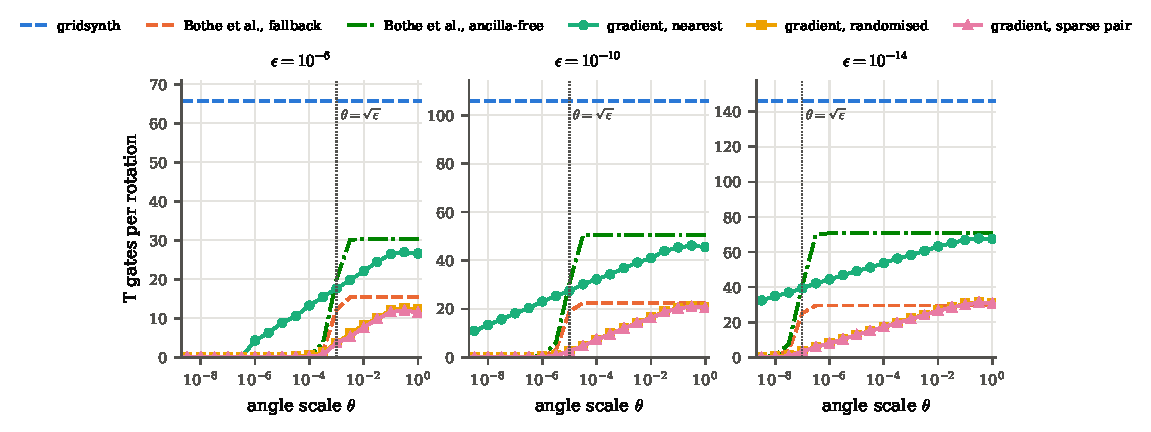
\includegraphics[width=\textwidth]{../figures/fig_layer.pdf}
\caption{T gates per rotation in a layer of $L=1024$ rotations, in batches of at most 256
signed digits, against
the angle scale $\theta$ (angles log-uniform in $[\theta/2,\theta]$, random signs), at three
per-rotation errors. Dashed: gridsynth (fit to runs), flat in $\theta$, and the angle-dependent
costs of Bothe \textit{et al.}~\cite{Bothe2026} on the same angles, flat down to
$\theta\approx\sqrt\epsilon$ and falling steeply below. The gradient's cost falls by about one T
gate per halving of the angle over the whole range above $\sqrt\epsilon$.}
\label{fig:layer}
\end{figure*}

\paragraph*{One layer.}
Figure~\ref{fig:layer} shows the cost per rotation in a layer of 1,024 rotations. At
$\epsilon=10^{-10}$, randomised rounding onto sparse pairs ($b=18$) uses 20.5 T gates per
rotation for angles of order one, 16.2 at $10^{-2}$, 7.3 at $10^{-4}$ and 2.6 at $10^{-5}$.
Bothe \textit{et al.}'s fallback scheme uses 22.5 at all of these but the last, where it is 18.9,
and their ancilla-free scheme 50.5 and 30.6. Below $\theta\approx\sqrt\epsilon=10^{-5}$ both
costs collapse: 0.65 against 2.84 at $3\times10^{-6}$, 0.09 against 0.28 at $10^{-6}$, and then
0.05 against 0.02 at $3\times10^{-7}$, where theirs is the smaller. At $\epsilon=10^{-14}$ and
$10^{-6}$ the picture is the same; the crossing, where there is one, lies below
$\sqrt\epsilon/10$. So the gradient wins by a factor that grows as the angle falls from one
towards $\sqrt\epsilon$, and synthesis wins well below it, at a few hundredths of a T gate. For
angles of order one the two are close: 9 per cent apart at $\epsilon=10^{-10}$, and at
$\epsilon=10^{-14}$ the gradient is 4 per cent worse (30.7 against 29.5). Plain randomised
rounding, onto adjacent grid points, agrees with sparse pairs down to $\sqrt\epsilon$ and costs
more below (0.31 against 0.09 at $10^{-6}$).

Nearest rounding ($b=35$) uses 45.6 T gates per rotation at angles of order one, 41.0 at
$10^{-2}$, 32.2 at $10^{-4}$ and 23.0 at $10^{-6}$, against 106 for gridsynth and 40.0 for the
unmixed fallback protocol. Its cost falls by about one T gate per halving of the angle, a little
below the $4/3$ of the digit count because the digits in the top three columns cost one T gate
or none.

\begin{figure}[t]
\centering
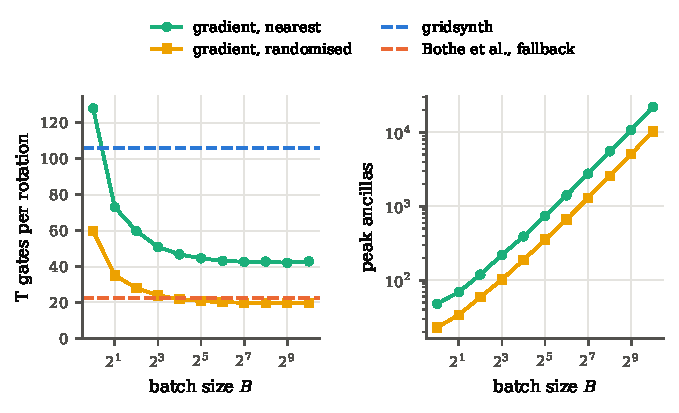
\includegraphics[width=\columnwidth]{../figures/fig_batch.pdf}
\caption{The batch size. Left: T gates per rotation at $\epsilon=10^{-10}$, angles in
$[0.05,0.1]$. A batch of one is a single rotation (Proposition~\ref{prop:one}) and is worse than
synthesis; two rotations already beat gridsynth, and sixteen match Bothe \textit{et al.}'s
fallback scheme, which at these angles is the mixed fallback cost. Right: peak ancillas, besides
the gradient register, which grow linearly with $B$.}
\label{fig:batch}
\end{figure}

\paragraph*{Batches and qubits.}
The addition's $b-2$ Toffolis are shared by a batch, and the ancillas grow with it
(Fig.~\ref{fig:batch}). With $B=1$, nearest rounding costs 128 T gates against gridsynth's 106,
and randomised rounding 59.7 against 22.5 for synthesis: Proposition~\ref{prop:one} in numbers.
With $B=2$ nearest rounding is already at 73; with $B=16$ the costs are 46.8 and 21.8 with 389
and 187 ancillas, and with $B=64$, 43.2 and 20.2 with 1,402 and 662. Beyond $B=64$ nothing is
gained. Batches of 256 digits, as in the other runs, cost 45.6 and 20.5 with 541 and 527
ancillas. The ancillas are the copies of the digit bits and the carries
(Theorem~\ref{thm:layer}); we have not tried to reduce them.

\begin{figure*}[t]
\centering
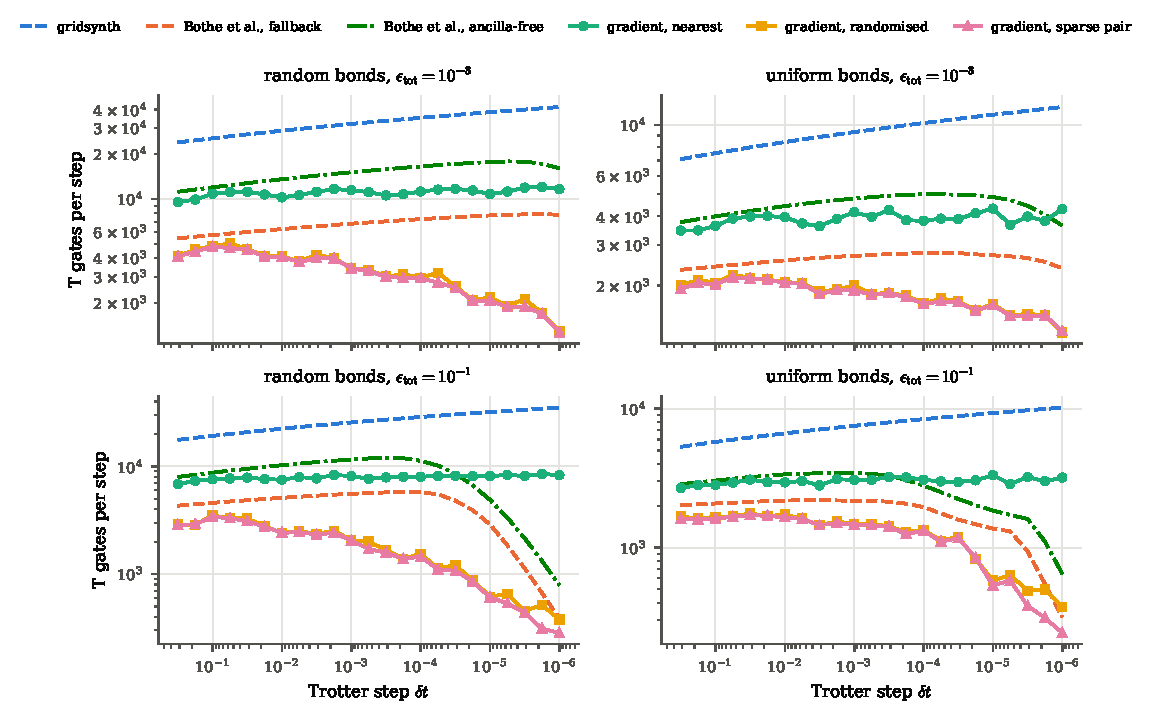
\includegraphics[width=\textwidth]{../figures/fig_trotter.pdf}
\caption{T gates per second-order Trotter step of a Heisenberg chain of 64 spins in a random
field, run to $t=10$, against the step $\delta t$, at total synthesis errors of $10^{-3}$ (top)
and $10^{-1}$ (bottom). Left: random bonds, every angle distinct. Right: uniform bonds, where
each method uses Hamming-weight phasing if it is cheaper. The total is the step cost times
$10/\delta t$ steps. Synthesis by Bothe \textit{et al.}'s formulas gets dearer as the step shrinks
until the angles reach $\sqrt\epsilon$, then cheaper; the gradient layers get cheaper throughout.}
\label{fig:trotter}
\end{figure*}

\paragraph*{A Trotter simulation.}
Take an open chain of $n=64$ spins,
\begin{equation}
  H=\sum_{i=1}^{n-1}J_i\,(X_iX_{i+1}+Y_iY_{i+1}+Z_iZ_{i+1})+\sum_{i=1}^nh_iZ_i,
\end{equation}
with $h_i$ uniform in $[-1,1]$, and either random bonds $J_i$ uniform in $[0.5,1.5]$ or uniform
bonds $J_i=1$. The $XX$ terms commute with each other, as do the $YY$ terms and the $ZZ$ and
field terms, so a second-order step is four layers, $XX(\delta t)\,YY(\delta t/2)\,[ZZ+Z]
(\delta t)\,YY(\delta t/2)$, with the half steps of $XX$ merged across steps. We run to $t=10$,
so $r=10/\delta t$ steps, at a total synthesis error $\epsilon_{\rm tot}$ of $10^{-3}$ or
$10^{-1}$, split evenly over the $R$ approximated rotations of each step: $R=4(n-1)+n=316$ with
random bonds. With uniform bonds a method may first sum each class of 63 equal angles into its
Hamming weight, and then needs one rotation per bit of it, $R=4\cdot6+n=88$, at the cost of the
Hamming-weight tree; each method, synthesis and gradient alike, takes whichever of the two is
cheaper at each step. The Trotter error itself, which sets $\delta t$, is outside the comparison;
Fig.~\ref{fig:trotter} gives the cost of whatever step is chosen, with batches of at most 256
digits and the gradient's costs averaged over five draws of the roundings. The steps run from $0.3$ to
$10^{-6}$, so the per-rotation errors run from $4\times10^{-5}$ to $3\times10^{-13}$ and the angles from about
$0.5$ to $10^{-6}$: the small-angle regime $\theta^2\lesssim\epsilon$ is reached only at the
smallest steps of the looser budget.

At $\epsilon_{\rm tot}=10^{-3}$ with random bonds, the gradient layers (sparse pairs) use $0.76$
times the T gates of Bothe \textit{et al.}'s fallback scheme at $\delta t=0.3$, $0.61$ at
$3\times10^{-3}$, $0.34$ at $3\times10^{-5}$ and $0.16$ at $10^{-6}$. At $\delta t=10^{-3}$ the
whole run costs $6.81\times10^7$ T gates by their fallback scheme, $1.51\times10^8$ by their
ancilla-free scheme, $3.19\times10^8$ by gridsynth, and $3.41\times10^7$ with the gradient. With
uniform bonds, where Hamming-weight phasing already takes much of the cost, the ratio runs from
$0.83$ to $0.53$. At $\epsilon_{\rm tot}=10^{-1}$ the ratios fall to $0.20$ with random bonds and
$0.39$ with uniform bonds; here the smallest steps reach the regime where synthesis falls as
$\theta^2/\epsilon$, and the ratio climbs back to $0.74$ and $0.77$ at $\delta t=10^{-6}$. Over
all four cases and all 23 steps the gradient never uses more T gates than Bothe
\textit{et al.}'s fallback scheme; the ratio lies between $0.16$ and $0.88$. Randomised rounding
onto adjacent grid points does lose at the smallest steps of the looser budget, by up to a
factor of $1.19$: there the sparse pairs matter. Sending each rotation to whichever of the two
methods has the lower expected cost, judged per rotation before the draw, changed the totals by
$-7$ to $+12$ per cent: the per-rotation estimate misses the shared addition and the
Hamming-weight tree. We do not show it; a better router would judge whole batches. Nearest
rounding uses $0.24$ to $0.51$ times the T gates of gridsynth. The ancillas peak at 589 for the
randomised layers and 656 for nearest rounding.

% ----------------------------------------------------------------------------------------------
\section{Discussion}\label{sec:discussion}

So the answer to the question we started with is that a phase gradient does not make a
rotation cheaper, but it makes a layer of rotations cheaper, because it turns the precision of
each angle into a cost per nonzero digit and pays for the carry chain once per layer. The cost
of a rotation is then about four T gates per signed digit, so it depends on
$\log_2(\theta/\Delta)$ rather than on $\log_2(1/\epsilon)$, and randomised rounding halves the
number of digits by halving $\log_2(1/\Delta)$. Angle-dependent synthesis~\cite{Bothe2026} and
the gradient exploit small angles in different ranges: synthesis below $\sqrt\epsilon$, where a
rotation is mostly the identity, and the gradient everywhere above it, where synthesis still
pays the full $0.53\log_2(1/\epsilon)$. Most rotations of a Trotter step at a useful precision
are in the second range, and there the gradient wins by a factor of up to six in our examples.

Several things are not in the comparison.
\begin{itemize}
\item \emph{T gates only.} We count T gates and ancillas. We have not laid out the circuits,
  scheduled them or counted their depth. The \AND{}s of a column reduction are sequential within
  a column; the additions are a carry chain of $b-2$ Toffolis. Synthesised rotations are
  sequences of T gates on one qubit, and they parallelise across the layer.
\item \emph{Toffolis as four T gates.} With a catalysed CCZ factory a Toffoli costs about as
  much as two T gates~\cite{Gidney2019}, which would roughly halve the gradient's counts. We
  have not used this.
\item \emph{Synthesis costs are formulas.} We evaluate the formulas of
  Refs.~\cite{Bothe2026,Kliuchnikov2023} on our angles; we have not run their methods. The
  fallback scheme's small-angle term is their substitution $\epsilon\to2\epsilon$ in the
  ancilla-free one.
\item \emph{Quasi-probabilities.} Bothe \textit{et al.}'s largest savings come from
  quasi-probability mixtures with a total $\lambda$ of order one, which cost a constant factor
  in samples instead of an error. Randomised rounding onto the gradient could be given negative
  weights in the same way; we have not done it, and do not compare in that setting.
\item \emph{Ancillas.} A batch of 256 digits needs 500 to 660 ancillas, most of them copies of
  digit bits and carries kept until the uncompute. Smaller batches trade them for the share of
  the addition (Fig.~\ref{fig:batch}). A layer whose bits were reduced in place, or whose
  columns were streamed, would need fewer; we have not tried. Synthesis needs none (or one, for
  fallback).
\item \emph{Equal angles.} When a layer has many equal angles, Hamming-weight phasing does most
  of the work and the gradient adds less (the uniform chain). Angles that share digits but are
  not equal, as in a Fourier series of coefficients, could share partial sums across columns;
  we have not looked at this.
\item \emph{The gradient register.} It needs $b$ qubits and $b-3$ synthesised rotations, once.
  Its error enters once. We have not included either.
\end{itemize}

The construction is the oldest trick in multiplier design, a column reduction of partial
products~\cite{Wallace1964}, put in front of the phase-gradient adder; and its parts, the
measured \AND{}~\cite{Jones2013,Gidney2018}, Hamming-weight
phasing~\cite{Gidney2018,Kivlichan2020}, weighted sums of bits into a gradient~\cite{Sanders2020,
Dutta2026}, and mixing~\cite{Hastings2017,Campbell2017}, are all known. What we have added is
the observation that for fixed angles the reduction can run over signed digits, the count that
follows from it, and the comparison with angle-dependent synthesis that shows where it pays:
for angles between about $\sqrt\epsilon$ and one, once a batch holds a few rotations, which is
where most of a Trotter step lies.

\paragraph*{Code availability.}
The code that compiles the layers, simulates them, counts them and makes the figures, with its
tests and data, is in Ref.~\cite{code}, directory \texttt{phasegrad\_trotter}.

\bibliography{refs}

\end{document}
